\documentclass[final]{beamer}
%% based on the Dreuw style
\mode<presentation>
{
	\setbeamertemplate{block begin}{
		\vskip.25ex
		\begin{beamercolorbox}[rounded=true,shadow=true,leftskip=1cm,colsep*=.75ex]{block title}%
			\usebeamerfont*{block title}\insertblocktitle
		\end{beamercolorbox}%
		{\ifbeamercolorempty[bg]{block body}{}{\nointerlineskip\vskip-0.5pt}}%
		\usebeamerfont{block body}%
		\begin{beamercolorbox}[rounded=true,shadow=false,colsep*=.75ex,sep=.75ex,vmode]{block body}%
			\ifbeamercolorempty[bg]{block body}{\vskip-.25ex}{\vskip-.75ex}\vbox{}%
		}
		\setbeamertemplate{block end}{
		\end{beamercolorbox}
	}
	\setbeamertemplate{headline}{
		\leavevmode
		
		\begin{beamercolorbox}[wd=\paperwidth]{headline}
			\begin{columns}[T]
				\begin{column}{.02\paperwidth}
				\end{column}
				\begin{column}{.22\paperwidth}
					\begin{center}
						
\includegraphics[scale=0.1]{transparentStatisticsLaura201617.jpg}
						
\includegraphics[scale=0.16]{nsf.png}
					\end{center}
					\vskip0.5ex
				\end{column}
				\begin{column}{.675\paperwidth}
					\vskip4ex
					\raggedleft
					\usebeamercolor{title in headline}{\color{fg}\textbf{\LARGE{\inserttitle}}\\[1ex]}
					\usebeamercolor{author in headline}{\color{fg}\large{\insertauthor}\\[1ex]}
					\usebeamercolor{institute in headline}{\color{fg}\large{\insertinstitute}\\[1ex]}
				\end{column}
				\begin{column}{.1\paperwidth}
					\vskip1cm
					\begin{center}
						
\includegraphics[scale=0.5]{Purduelogo.jpg}
					\end{center}
					\vskip1.5cm
				\end{column}
				\begin{column}{.03\paperwidth}
				\end{column}
			\end{columns}
		\end{beamercolorbox}
		
		\begin{beamercolorbox}[wd=\paperwidth]{lower separation line head}
			\rule{0pt}{2pt}
		\end{beamercolorbox}
	}
}
\usecolortheme{purduegold}
\usepackage{times}
\usepackage{tikz}
\usepackage{pgfplots}
\pgfplotsset{compat=1.5}
\usepackage{siunitx}
\usetikzlibrary{calc}
\usepackage{amsmath,amsthm, amssymb, latexsym}
\boldmath
\usepackage[english]{babel}
\usepackage[latin1]{inputenc}
\usepackage[size=custom,width=121.2,height=91.2, scale=1.2,debug]{beamerposter}

\usepackage[round]{natbib}
\usepackage{graphicx}
\usepackage{url}
\usepackage{bm}

\usepackage{lipsum}  

\graphicspath{{figures/}}
\title[Fancy Posters]{Rates of DNA Mutation in Genes and Inte-Gene Regions}
\author{Brian French, Nicole Markley, Laszlo Csonka, and Mark Daniel Ward}
\institute{Department of Biology, Purdue University, West Lafayette, IN}
%  \date{March 25, 2016}

\begin{document}
	\begin{frame}{}
	\begin{columns}[t]
		
		%%%%%%%%%%%%%%%%%%%%%%%%%%%%%%%%%%%%%%%%%%%%%%%%%%%%%%%%%%%%%%%%%%%%%%
		
		\begin{column}{.32 \linewidth}
			\begin{block}{\large Abstract}
				The aim of our analysis was to compare the rates of evolution of DNA sequences of genes and intergenic regions. The chromosomes of the related genera of bacteria, Escherichia coli K-12, Salmonella enterica serovar Typhimurium, and Citrobacter koseri, contain extensive regions in which the order of genes of identical. The fact that the gene order is so conserved suggests that both the genes and intergenic spacers were derived by evolution from corresponding sequences in the last common ancestor of the three organisms, and it enabled us to compare the sequence changes in functional genes and in intergenic spacers across the three organisms.
				\newline
				\newline
				Pairwise comparisons using BLASTN were used to identify regions that had shared genes. ClustalW was then used to identify single base mutations in both genes and inter-gene regions. Mutation frequencies were determined for all paired comparisons. This analysis indicated that the mutation frequencies are significantly higher in intergenic spacers do not have specific sequence-dependent functions, and therefore, they can accumulate mutations more liberally than genes, which are constrained by their function.
			\end{block}
			
			\begin{block}{\large Background}
				\begin{itemize}
					\item Genomes have both useful genetic information coded in genes and presumed useless inter-gene regions termed as gaps.
					\item Gene pairs between organisms can be isolated using a tool called \textbf{B}asic \textbf{L}ocal \textbf{A}lignment \textbf{S}earch \textbf{T}ool, commonly referred to as BLAST. 
					
					\item \textit{Salmonella Typhimurium LT2}, \textit{Citrobacter Koseri}, and \textit{Escherchia Coli MG1655} were chosen because they are closely related members of \textit{Enterobacteriaceae}.
					\newline
					\includegraphics[scale = 1]{phylogeny.png}
					\newline
					\item The phylogeny tree built from 16s rRNA shows the relative relations of the three bacteria chosen to be analyzed, which is an explanation of why E. Coli and Citrobacter have smaller common regions than Citrobacter and Salmonella.
				\end{itemize}
			\end{block}
			
			\begin{block}{\large Motivation}
				
				\begin{itemize}
					
					\item Mutation in genes has a double constrainment of DNA's built in error-handling as well as maintenance of gene function. 
					
					\item Gaps are presumed to have no function, so they should mutate faster and more randomly.  
					
					\item Choosing pairs of bacteria that were closely related could be used to infer rates of mutation in homologous genes and gap regions. 
					
					\item Differing rates of mutation would suggest that gaps don't share genes' constrainment due to function.
				\end{itemize}
			\end{block}
			
			\begin{block}{\large Question}
				\begin{itemize}
					\item Do gaps and genes mutate in the same way?
					\item Is this trend consistent in different pairs of bacteria?
					\item Do mutations show any form of dependence on other mutations?
				\end{itemize} 
			\end{block}
			
			
			
		\end{column}
		
		%%%%%%%%%%%%%%%%%%%%%%%%%%%%%%%%%%%%%%%%%%%%%%%%%%%%%%%%%%%%%%%%%%%%%%
		
		\begin{column}{.32 \linewidth}
			\begin{block}{\large Hypothesis}
				We hypothesize that genes will mutate at different rates than gaps because they have to code information essential to cell survival.
				
			\end{block}
			\begin{block}{\large Illustrations}
				Figure 1
				\newline
				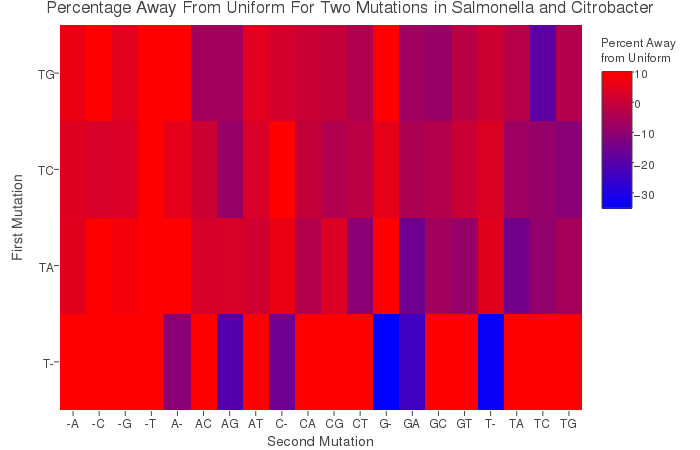
\includegraphics[scale = 1.9]{thursVersion.jpeg}
				\newline
				Figure 2
				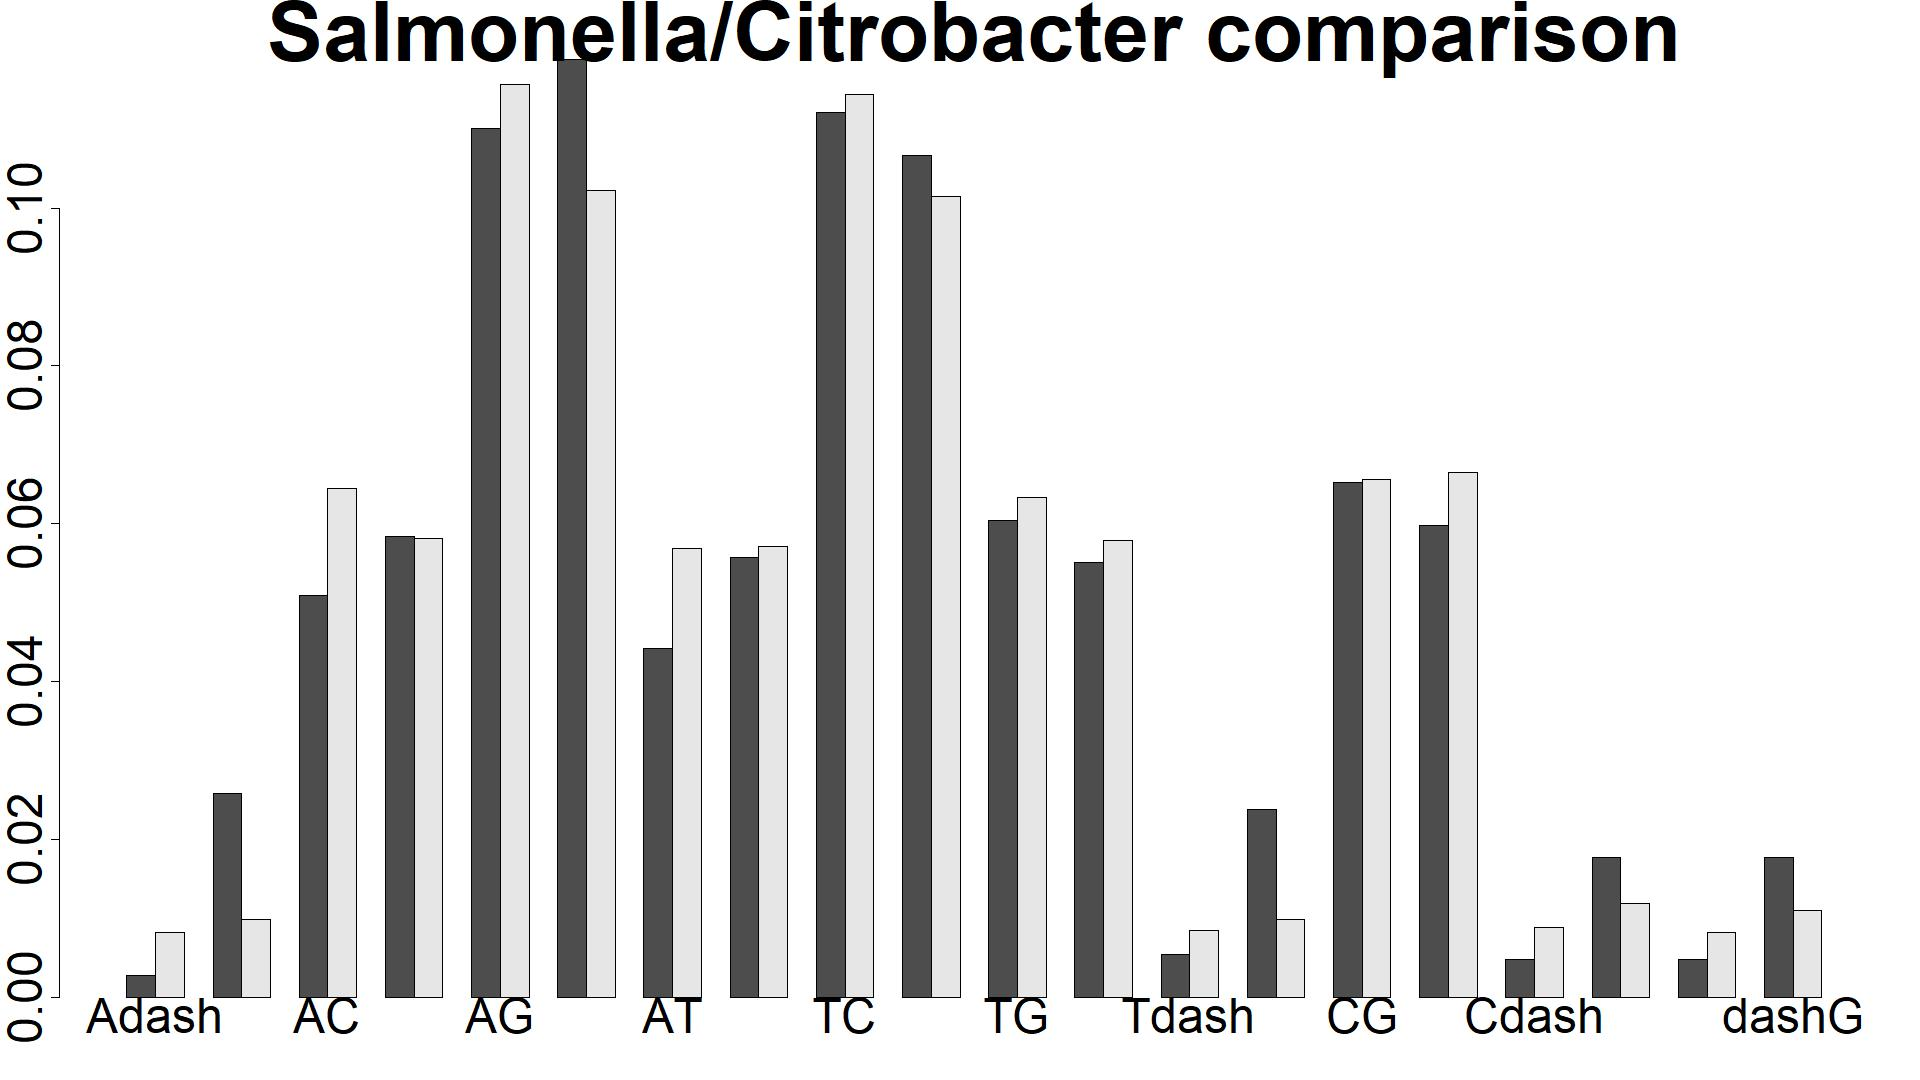
\includegraphics[scale = .55]{CBSalPercentage.jpeg}
				\newline
				Figure 3
				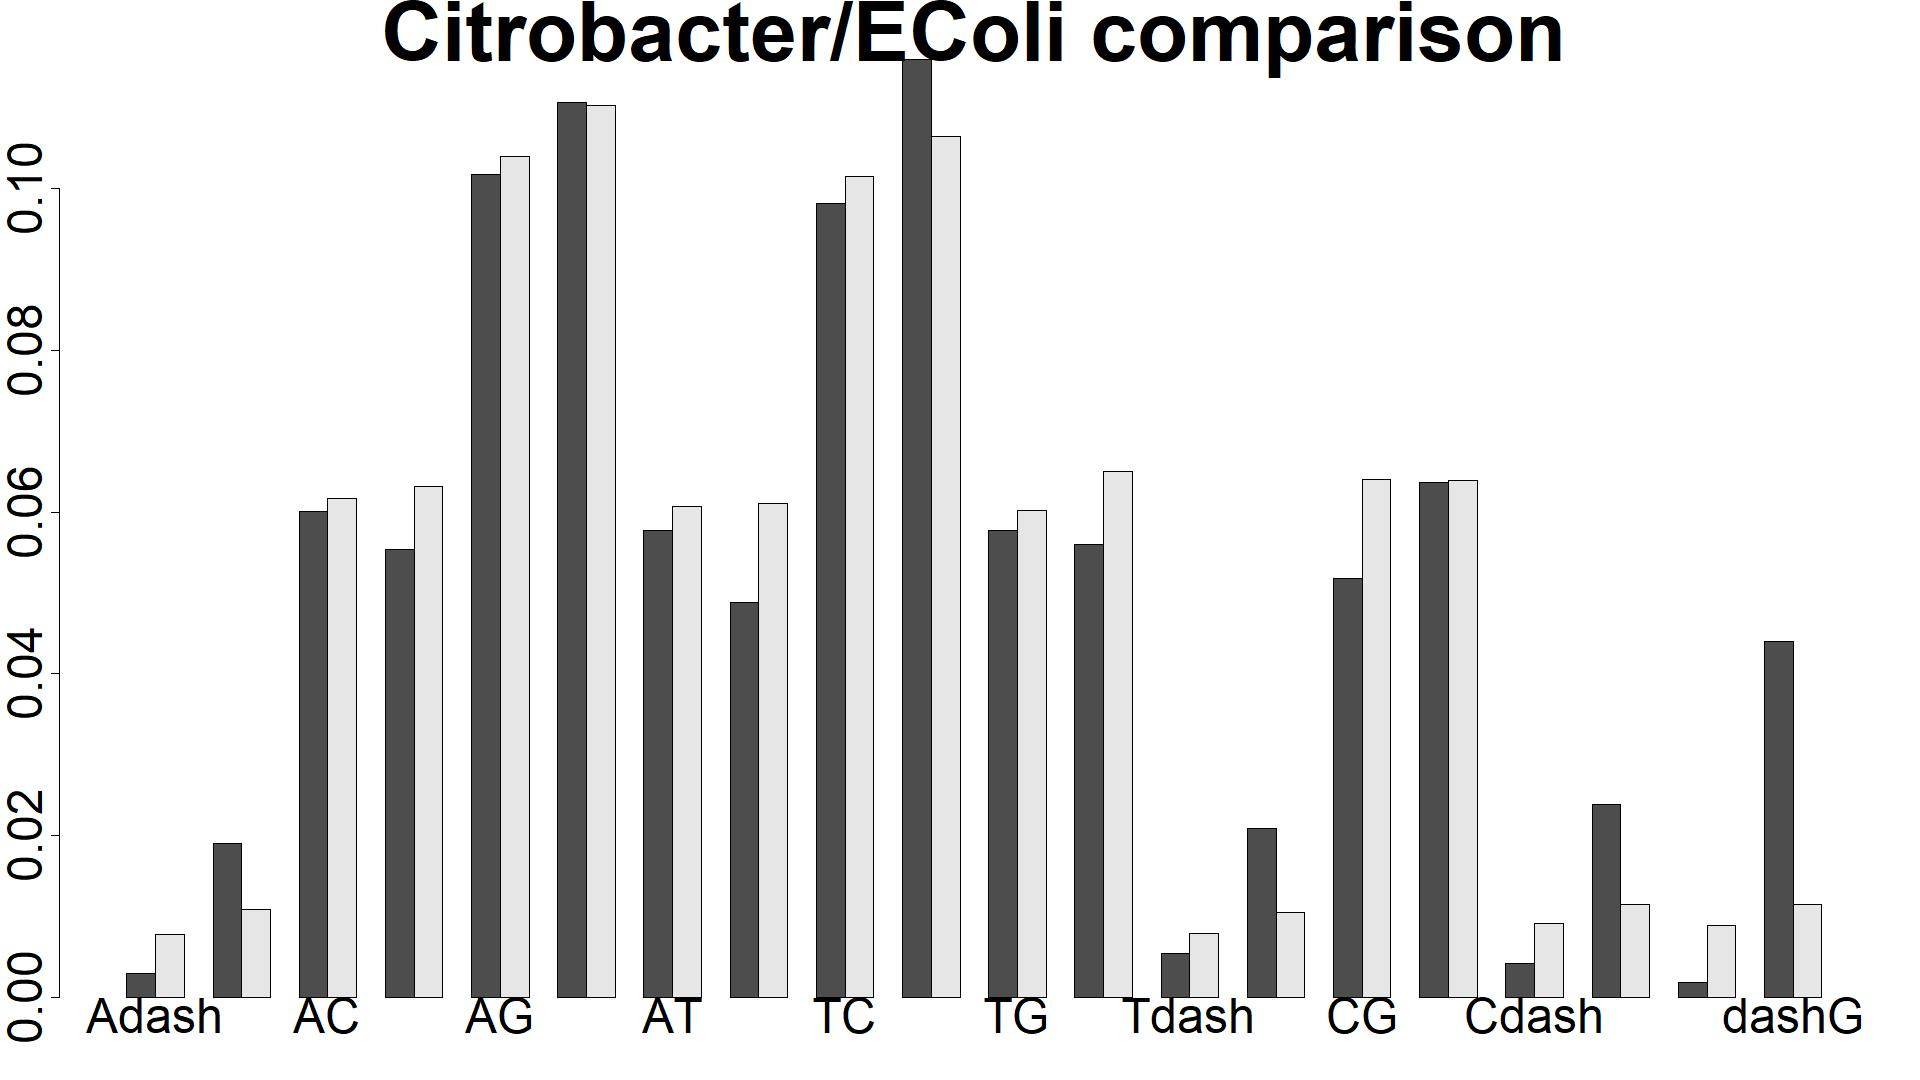
\includegraphics[scale = .55]{CBECPercentage.jpeg}
				
				
			\end{block}
			
			
		\end{column}
		
		
		
		%%%%%%%%%%%%%%%%%%%%%%%%%%%%%%%%%%%%%%%%%%%%%%%%%%%%%%%%%%%%%%%%%%%%%%
		
		\begin{column}{.32 \linewidth}
			
			\begin{block}{Procedure}
				Genomes were run through BLAST to identify matching regions for each pair comparison. BLAST matches were presumed to be homologous genes. Two matching regions with a non-matching region between them led the non-matching region to be labeled as a gap. Any gap longer than 500 bases was presumed to contain a gene that wasn't present in the compared genome and was therefore discarded.
				\newline
				Matched regions (both genes and gaps) were run through CLUSTALw and any base mismatch preceded and followed by at least 3 matching bases was presumed to be a mutation. Mutation rates were then tabulated, plotted, and chi-squared tested on mutation counts.
			\end{block}
			\begin{block}{\large Conclusion}
				\begin{itemize}
					\item Purine->purine and pyrimidine->pyrimidine mutations were more frequent than other possible single base-pair changes both in genes and in gaps, indicating that single-base changes were not random.
					\item 
					Genes and gaps have statistically different mutation rates as shown by a chi-square test (p $<$ \num{2.2} * \num{10e-16}) in all three gene pairs
					\item This suggests that genes and gaps have different mutation patterns
					\item When insertions and deletions are removed, there's a large drop in statistical significance, which indicates that a major part of the difference is gaps losing information.
					\item When insertions and deletions are removed, E. coli and Salmonella have the smallest change in significance, indicating that there are more base shift mutations in gaps than genes in that pair.
					\item In the case of two mutated bases next to each other, there is Markovian dependence in genes
					\item There were insufficient examples of two mutated bases that were adjacent to each other was in gaps to enable us to draw conclusions about their dependence.
					
				\end{itemize}
				
				
				
			\end{block}
			
			
			%%% If you know how to use BibTeX
			%%%	  \begin{block}{\large References}
			%%%	  \vspace{-.5cm} \footnotesize
			%%%	\bibliographystyle{abbrvnat}     % mathematics and physical sciences
			%%%	\bibliography{forbidden}   % name your BibTeX data base
			%%%	\vspace{-.25cm}
			%%%	 \end{block}
			
			\begin{block}{Acknowledgments}
				This research is supported by NSF grant DMS \#1246818 and NSF grant \# IOS-1456829
			\end{block}
			\begin{block}{Citations}
				\footnotesize
				Thompson, J. D., Gibson, T. J. and Higgins, D. G. 2002. Multiple Sequence Alignment Using ClustalW and ClustalX. Current Protocols in Bioinformatics. 00:2.3:2.3.1?2.3.22.
				
				Stephen F. Altschul, Warren Gish, Webb Miller, Eugene W. Myers, David J. Lipman, Basic local alignment search tool, Journal of Molecular Biology, Volume 215, Issue 3, 1990, Pages 403-410, ISSN 0022-2836, http://dx.doi.org/10.1016/S0022-2836(05)80360-2.
				(http://www.sciencedirect.com/science/article/pii/S0022283605803602)
				BLAST accessed through https://blast.ncbi.nlm.nih.gov/Blast.cgi
				
			\end{block}
			\begin{block}{Dot Plot Representation of Salmonella/EColi Gene Locations}
				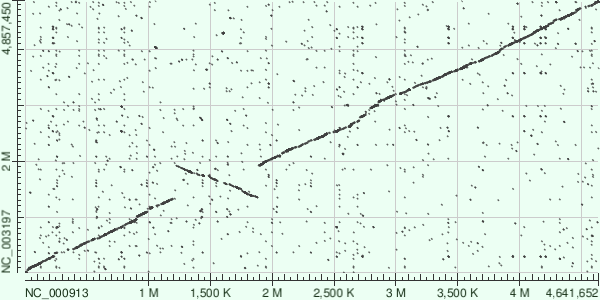
\includegraphics[scale = 1.25]{hit_matrixECSal.png}
			\end{block}
			
			
			
		\end{column}
		
	\end{columns}
	
\end{frame}
\end{document}	



